%%%%%%%%%%%%  Generated using docx2latex.com  %%%%%%%%%%%%%%

%%%%%%%%%%%%  v2.0.0-beta  %%%%%%%%%%%%%%

\documentclass[12pt]{article}
\usepackage{amsmath}
\usepackage{latexsym}
\usepackage{amsfonts}
\usepackage[normalem]{ulem}
\usepackage{soul}
\usepackage{array}
\usepackage{amssymb}
\usepackage{extarrows}
\usepackage{graphicx}
\usepackage[backend=biber,
style=numeric,
sorting=none,
isbn=false,
doi=false,
url=false,
]{biblatex}\addbibresource{bibliography-biblatex.bib}

\usepackage{subfig}
\usepackage{wrapfig}
\usepackage{wasysym}
\usepackage{enumitem}
\usepackage{adjustbox}
\usepackage{ragged2e}
\usepackage[svgnames,table]{xcolor}
\usepackage{tikz}
\usepackage{longtable}
\usepackage{changepage}
\usepackage{setspace}
\usepackage{hhline}
\usepackage{multicol}
\usepackage{tabto}
\usepackage{float}
\usepackage{multirow}
\usepackage{makecell}
\usepackage{fancyhdr}
\usepackage[toc,page]{appendix}
\usepackage[hidelinks]{hyperref}
\usetikzlibrary{shapes.symbols,shapes.geometric,shadows,arrows.meta}
\tikzset{>={Latex[width=1.5mm,length=2mm]}}
\usepackage{flowchart}\usepackage[paperheight=11.0in,paperwidth=8.5in,left=1.0in,right=1.0in,top=1.2in,bottom=0.30000000000000004in,headheight=1in]{geometry}
\usepackage[utf8]{inputenc}
\usepackage[T1]{fontenc}
\TabPositions{0.5in,1.0in,1.5in,2.0in,2.5in,3.0in,3.5in,4.0in,4.5in,5.0in,5.5in,6.0in,}

\urlstyle{same}

\renewcommand{\_}{\kern-1.5pt\textunderscore\kern-1.5pt}

 %%%%%%%%%%%%  Set Depths for Sections  %%%%%%%%%%%%%%

% 1) Section
% 1.1) SubSection
% 1.1.1) SubSubSection
% 1.1.1.1) Paragraph
% 1.1.1.1.1) Subparagraph


\setcounter{tocdepth}{5}
\setcounter{secnumdepth}{5}


 %%%%%%%%%%%%  Set Depths for Nested Lists created by \begin{enumerate}  %%%%%%%%%%%%%%


\setlistdepth{9}
\renewlist{enumerate}{enumerate}{9}
		\setlist[enumerate,1]{label=\arabic*)}
		\setlist[enumerate,2]{label=\alph*)}
		\setlist[enumerate,3]{label=(\roman*)}
		\setlist[enumerate,4]{label=(\arabic*)}
		\setlist[enumerate,5]{label=(\Alph*)}
		\setlist[enumerate,6]{label=(\Roman*)}
		\setlist[enumerate,7]{label=\arabic*}
		\setlist[enumerate,8]{label=\alph*}
		\setlist[enumerate,9]{label=\roman*}

\renewlist{itemize}{itemize}{9}
		\setlist[itemize]{label=$\cdot$}
		\setlist[itemize,1]{label=\textbullet}
		\setlist[itemize,2]{label=$\circ$}
		\setlist[itemize,3]{label=$\ast$}
		\setlist[itemize,4]{label=$\dagger$}
		\setlist[itemize,5]{label=$\triangleright$}
		\setlist[itemize,6]{label=$\bigstar$}
		\setlist[itemize,7]{label=$\blacklozenge$}
		\setlist[itemize,8]{label=$\prime$}

\setlength{\topsep}{0pt}\setlength{\parindent}{0pt}

 %%%%%%%%%%%%  This sets linespacing (verticle gap between Lines) Default=1 %%%%%%%%%%%%%%


\renewcommand{\arraystretch}{1.3}


%%%%%%%%%%%%%%%%%%%% Document code starts here %%%%%%%%%%%%%%%%%%%%



\begin{document}


%%%%%%%%%%%%%%%%%%%% Figure/Image No: 1 starts here %%%%%%%%%%%%%%%%%%%%

\begin{figure}[H]
	\begin{Center}
		
\includegraphics[width=2.29in,height=0.87in]{./media/image1.png}
	\end{Center}
\end{figure}


%%%%%%%%%%%%%%%%%%%% Figure/Image No: 1 Ends here %%%%%%%%%%%%%%%%%%%%

\setlength{\parskip}{12.0pt}
\begin{adjustwidth}{-0.39in}{-0.57in}
\begin{Center}
\sout{\textcolor[HTML]{00796B}{$\ast$ }}
\end{Center}
\end{adjustwidth}

\section*{Group 4 AI Summative Project}
\addcontentsline{toc}{section}{Group 4 AI Summative Project}
\chapter{AI Statistical Prediction Model for Africa’s rate of Employment in Agriculture with respect to Education Attainment, Literacy Levels, employment and unemployment rate towards boosting Gross Domestic Product(GDP).}
\chapter{Prepared by }
\chapter{Joachim Wambua}
\chapter{Collins Nnamuka}
\chapter{Ephraim Adongo}
\chapter{Zuberi\  Msemo}

\vspace{\baselineskip}
\chapter{African Leadership University}
\chapter{Facilitator:Kudakwashe Dandajena}
\chapter{Course: Artificial Intelligence}
\chapter{Faculty: Computer Science}
\chapter{Date: April 2021}

\vspace{\baselineskip}

\vspace{\baselineskip}
\section*{AbstractArtificial Intelligence has in the recent past surfaced as the critical point to finding solutions to humanity’s evolving problems through accurate predictions allowing countries $\&$  organizations to prepare for possible future occurrences. With the tremendous recent advancements in AI and the immense influence it has had in other major industries globally, AI promises to solve Africa’s persisting challenges like unemployment rates, education, and often fluctuating GDP trends just to mention a few. Africa is the natural resource capital of the world, with all kinds of things ranging from minerals like Gold, diamonds, and bauxite to foodstuffs, timber cocoa, and many more which has been a safe zone for people without education to run to as a career path since it requires no certification or qualification. Africa, as it stands, has everything but has nothing; in the sense that we have all the basic resources to survive and build ourselves a fantastic world full of opportunities, but we lack the technical know-how and skills to rapidly improve in this rapidly changing world and make use of the natural resources we are blessed with. The leap into AI and technological advancement has propelled numerous countries out of poverty and low living standards.}
\addcontentsline{toc}{section}{AbstractArtificial Intelligence has in the recent past surfaced as the critical point to finding solutions to humanity’s evolving problems through accurate predictions allowing countries $\&$  organizations to prepare for possible future occurrences. With the tremendous recent advancements in AI and the immense influence it has had in other major industries globally, AI promises to solve Africa’s persisting challenges like unemployment rates, education, and often fluctuating GDP trends just to mention a few. Africa is the natural resource capital of the world, with all kinds of things ranging from minerals like Gold, diamonds, and bauxite to foodstuffs, timber cocoa, and many more which has been a safe zone for people without education to run to as a career path since it requires no certification or qualification. Africa, as it stands, has everything but has nothing; in the sense that we have all the basic resources to survive and build ourselves a fantastic world full of opportunities, but we lack the technical know-how and skills to rapidly improve in this rapidly changing world and make use of the natural resources we are blessed with. The leap into AI and technological advancement has propelled numerous countries out of poverty and low living standards.}
\begin{justify}
{\fontsize{9pt}{10.8pt}\selectfont Unemployment has often proven a tough challenge to beat especially in Africa for a number of reasons. However, as unemployment rises, the African population has taken drastic measures and either sought employment in the informal sectors or have become self-employed often in informal occupation roles like farming and livestock rearing labour. Our research focuses mainly on the correlation between unemployment amongst the African population and employment in the informal fields, agriculture to be precise. We also study other correlated features such as education levels, literacy, Labour force participation, and the Gross Domestic Product growth rate. \par}
\end{justify}
\section*{Keywords}
\addcontentsline{toc}{section}{Keywords}
{\fontsize{9pt}{10.8pt}\selectfont Artificial Intelligence, Gross Domestic Product, Agriculture, Resources, Education, Literacy, Unemployment, Labour force participation,\par}
\section*{1.0 Introduction}
\addcontentsline{toc}{section}{1.0 Introduction}
\chapter{1.1 Problem Background Context }
\begin{justify}
{\fontsize{9pt}{10.8pt}\selectfont The idea that humans have to live and meet their needs without compromising the ability of future generations to do the same has been the main focus of every country and continent since its introduction in 1987. Education and Unemployment have been in a worrying state in Africa for a long time, often because of debatable reasons such as politics and the lack of adequate educational resources. This has caused a steady rise in the rate of unemployment, affected the labour force participation between the formal and the informal sectors in African countries, leading to a gradual development process in Africa.\par}
\end{justify}

\vspace{\baselineskip}
\chapter{1.2 Problem Statement}
\begin{justify}
{\fontsize{9pt}{10.8pt}\selectfont Unemployment has been a persistent challenge for the African youth over the past 15 years where many African youths are seeking white-collar jobs and ignoring the informal jobs sectors and yet, the truth is that a large number of the population still dwell in the informal sectors specifically Agriculture [4]. Despite the informal sector, specifically, agriculture, becoming an important source of employment and the backbone of most economic activities in African countries, these informal jobs in agriculture still are not contributing enough towards boosting the African economy and consequently increasing the African GDP growth rate.\par}
\end{justify}
\begin{justify}
{\fontsize{9pt}{10.8pt}\selectfont Our\ core objective is to create a solution in the form of an AI model that predicts the growth or decline rate of the total number of employees in the informal sector(in this case agricultural sector) and how that correlates with factors such as levels of education, literacy levels and annual Growth Domestic Product(GDP) of African Countries.  \par}
\end{justify}

\vspace{\baselineskip}
\chapter{1.3 Objectives}
\begin{enumerate}
	\item {\fontsize{9pt}{10.8pt}\selectfont Identify a sustainable development challenge in Africa i.e how the rate of Agriculture unemployment in Africa affects the annual GDP of African countries.\par}
	\item {\fontsize{9pt}{10.8pt}\selectfont Develop an AI-based solution to the identified problem from an AI and Data Science Analysis.}
	\item {\fontsize{9pt}{10.8pt}\selectfont How viable can the proposed solutions be commercialized?}
	\item {\fontsize{9pt}{10.8pt}\selectfont Documenting the problem identification and solution process.}
	\item {\fontsize{9pt}{10.8pt}\selectfont Building a strong solution and recommendation to the problem.}
\end{enumerate}
\section*{2.0 Analysis Insights }
\addcontentsline{toc}{section}{2.0 Analysis Insights }
\textcolor[HTML]{666666}{2.1 General Analysis of Insights gained from the data}

\vspace{\baselineskip}
\begin{justify}
{\fontsize{9pt}{10.8pt}\selectfont The general analysis is based on the Dataset source as retrieved from the WorldBank Data website(\href{https://data.worldbank.org/}{\textcolor[HTML]{3C78D8}{\ul{https://data.worldbank.org/}}}) as CSV files and later be used to carefully do an Exploratory Analysis and generating Insights which are summarized as follows, \par}
\end{justify}

\vspace{\baselineskip}
\begin{justify}
{\fontsize{9pt}{10.8pt}\selectfont There is a high correlation(approximately 80$\%$ ) between Unemployment($\%$  of the total labour force), Employment in Agriculture ($\%$  of the total employment) $\&$  Education Attainment at least secondary level. This can be then attributed to the fact that the more African people who do not get higher education or no education at all would often end up diverting into informal occupation roles such as agriculture and farming as a form of self-employment. This causes high unemployment rates across the continent, meaning an increase in the illiteracy rate of the country and lowers the country’s GDP(Gross Domestic Product).\par}
\end{justify}


%%%%%%%%%%%%%%%%%%%% Figure/Image No: 2 starts here %%%%%%%%%%%%%%%%%%%%

\begin{figure}[H]
	\begin{Center}
		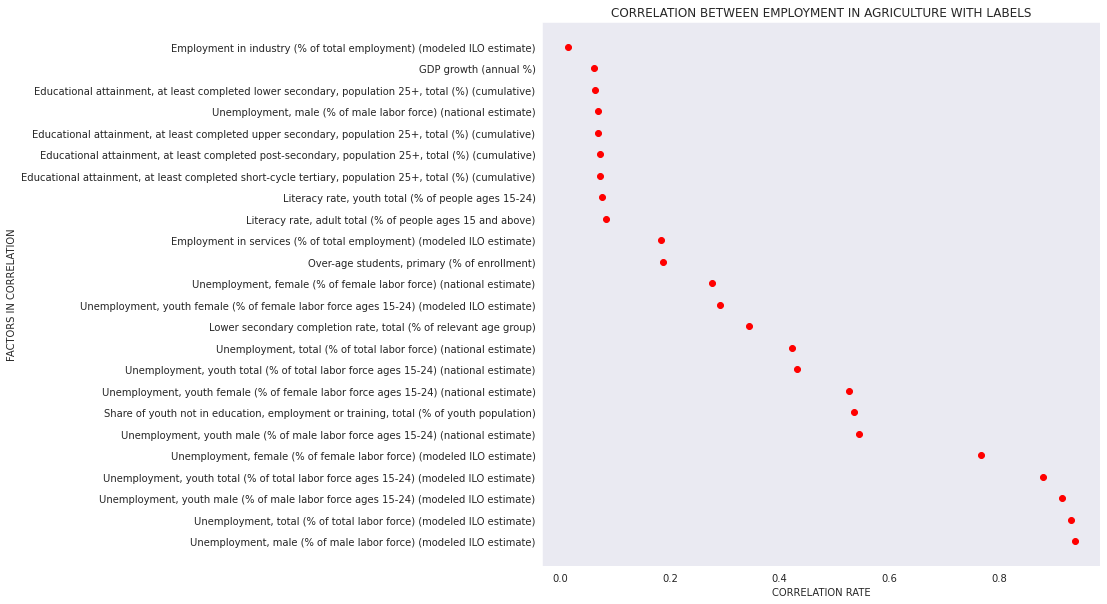
\includegraphics[width=6.21in,height=2.74in]{./media/image3.png}
	\end{Center}
\end{figure}


%%%%%%%%%%%%%%%%%%%% Figure/Image No: 2 Ends here %%%%%%%%%%%%%%%%%%%%


\vspace{\baselineskip}
\vspace{\baselineskip}
\begin{justify}
{\fontsize{8pt}{9.6pt}\selectfont \textit{Figure 1: Illustrates the correlation between Employment in agriculture Growth and different parameters around education levels, and gross domestic product.}\par}
\end{justify}

\vspace{\baselineskip}
\begin{justify}
{\fontsize{9pt}{10.8pt}\selectfont Furthermore, in our analysis, we found that there was some correlation(approximately 60$\%$ ) between education attainment (at least completed lower secondary) $\&$  literacy rates among the adults($\%$  of people age 15+) $\&$  youth($\%$  of people age 15 - 24) in Africa. We, therefore, inferred that the more African adults and youth who do not complete at least lower secondary education would eventually lead to a relatively higher African population of fairly illiterate masses. This category of the population is then referred to as people who engage in the Agricultural sector(informal sector) and possess little or inadequate expertise to positively influence the rise of gross domestic product(GDP).\par}
\end{justify}


%%%%%%%%%%%%%%%%%%%% Figure/Image No: 3 starts here %%%%%%%%%%%%%%%%%%%%

\begin{figure}[H]
	\begin{Center}
		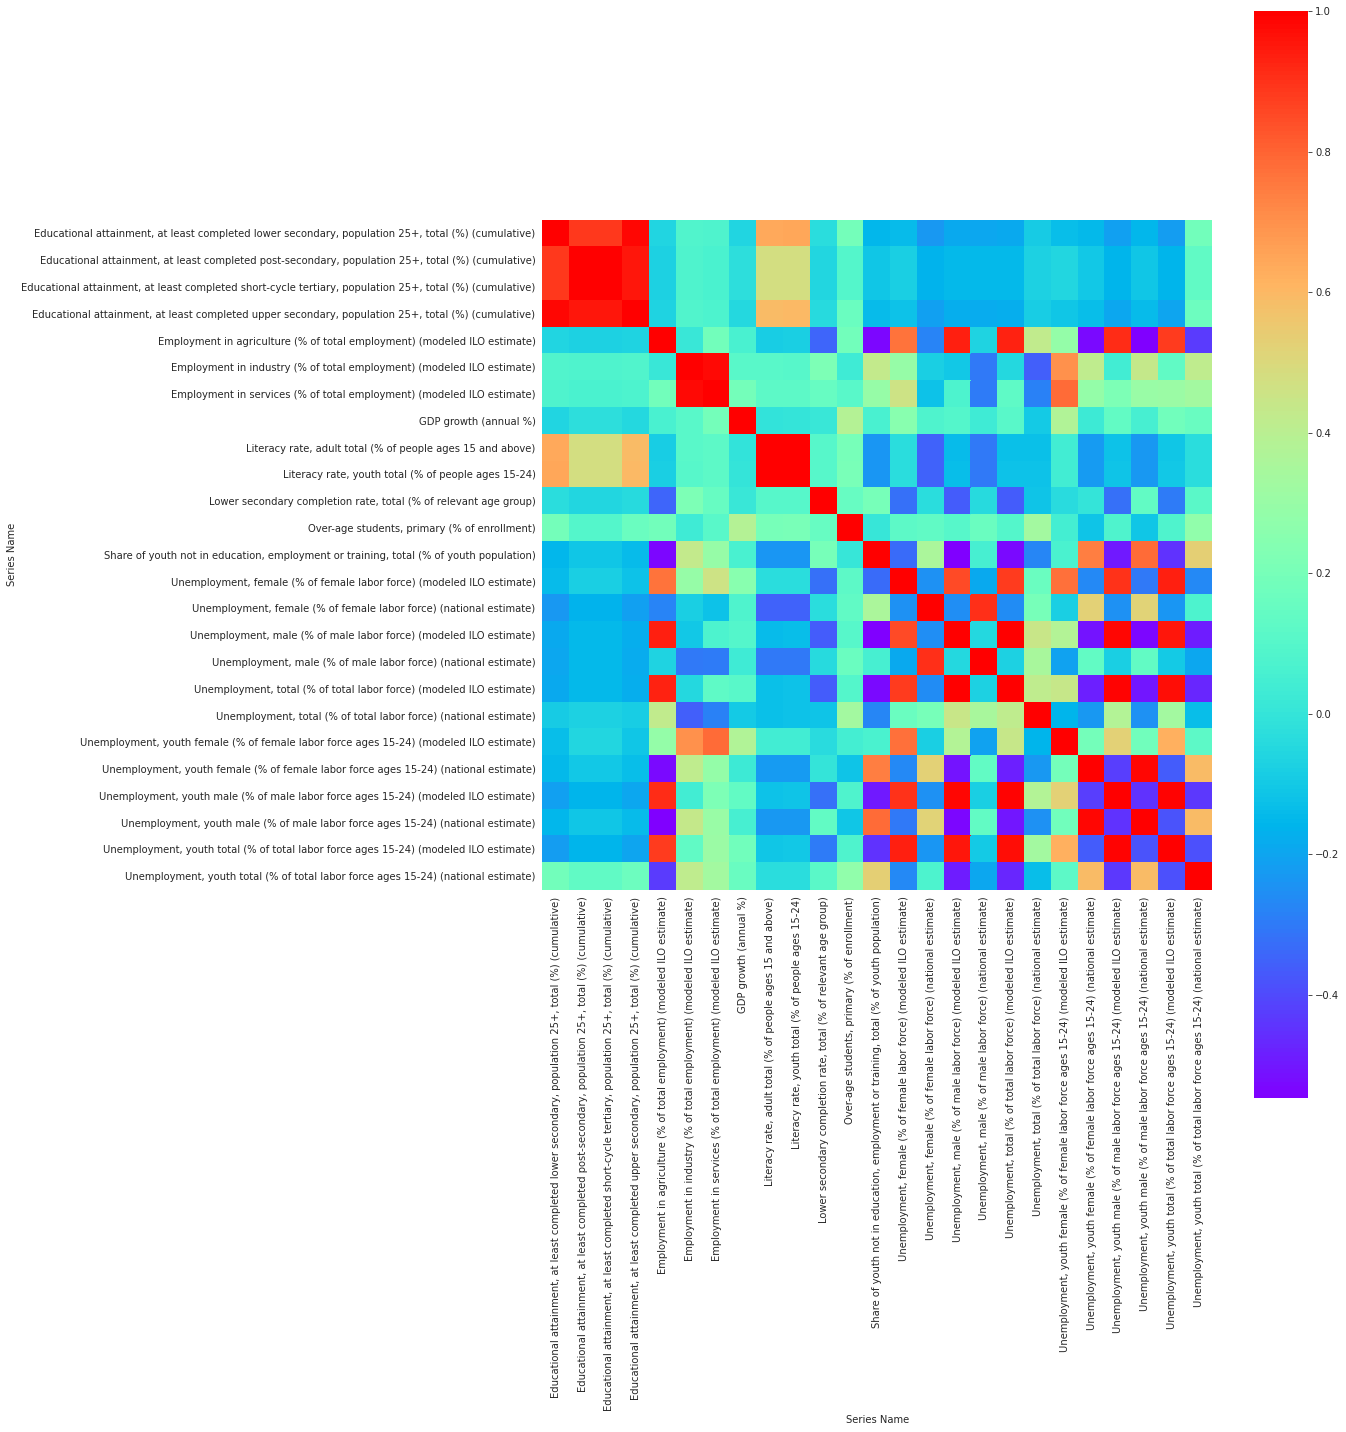
\includegraphics[width=6.95in,height=3.39in]{./media/image4.png}
	\end{Center}
\end{figure}


%%%%%%%%%%%%%%%%%%%% Figure/Image No: 3 Ends here %%%%%%%%%%%%%%%%%%%%


\vspace{\baselineskip}\begin{justify}
{\fontsize{8pt}{9.6pt}\selectfont \textit{Figure 3: A Broader Graph showing the correlation between the different features considered for this project.}\par}
\end{justify}

\vspace{\baselineskip}

\vspace{\baselineskip}
\begin{justify}
{\fontsize{9pt}{10.8pt}\selectfont We also observed a high correlation between the Share of youth not in education, employment or training($\%$  total of the youth population) and Unemployment in both male $\&$  female populations($\%$  of the total population). This means that a larger Africa population of citizens who take no part in education, training or employment, would eventually lead to a larger African population of unemployed citizens. We found this particular statistic worrying as it shows the need for more Africans to take up education, higher technical training, and employment so as to build better opportunities for future generations.\par}
\end{justify}

\vspace{\baselineskip}

\vspace{\baselineskip}


%%%%%%%%%%%%%%%%%%%% Figure/Image No: 4 starts here %%%%%%%%%%%%%%%%%%%%

\begin{figure}[H]
	\begin{Center}
		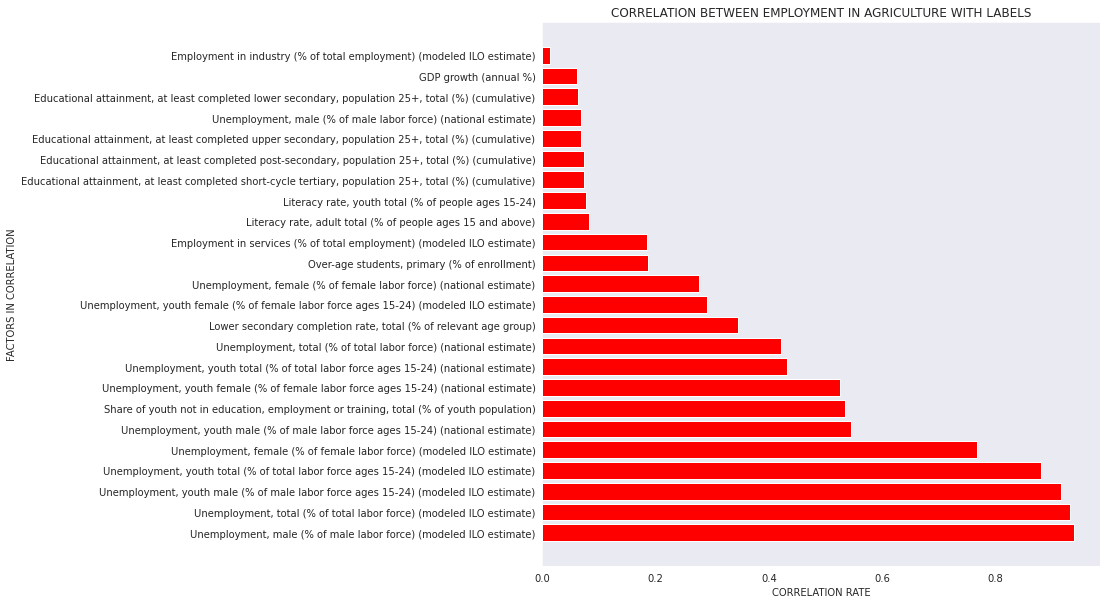
\includegraphics[width=6.47in,height=2.7in]{./media/image2.png}
	\end{Center}
\end{figure}


%%%%%%%%%%%%%%%%%%%% Figure/Image No: 4 Ends here %%%%%%%%%%%%%%%%%%%%


\vspace{\baselineskip}
\vspace{\baselineskip}
\begin{justify}
{\fontsize{8pt}{9.6pt}\selectfont \textit{Figure 2: A Correlation between Factors educational attainment and literacy rates with respect to other data points}\par}
\end{justify}
\section*{3.0 Proposed AI Solution}
\addcontentsline{toc}{section}{3.0 Proposed AI Solution}
\chapter{3.1\ \ \ \ AI Solution:  African Country Agriculture $\&$  Employment Trends Predictor and Optimizer Model:}
\begin{justify}
{\fontsize{9pt}{10.8pt}\selectfont From our dataset, we ran different regression models and correlation analyses. We found out that the factors; \textit{Unemployment rate, illiteracy rate (No education and secondary school level), }positively\ affect employment in agriculture, which also correlates to influence the growth in  GDP of countries at an average level of 91$\%$  accurate. We found this discovery very significant as it gave us a eureka moment for an AI solution.\par}
\end{justify}
\begin{justify}
{\fontsize{9pt}{10.8pt}\selectfont  }
\end{justify}
\begin{justify}
{\fontsize{9pt}{10.8pt}\selectfont \textit{Agriculture $\&$  Employment Trends Predictor and Optimizer Model} is an AI solution based model to predict the number of people to venture into informal sectors(agriculture and farming) based on the above-stated factors and to help draw the attention of the government, as to what it should focus on in order to improve their citizens’ living standards while boosting the African countries’ GDP growth rate.\par}
\end{justify}
\begin{justify}
{\fontsize{9pt}{10.8pt}\selectfont  }
\end{justify}
\begin{justify}
{\fontsize{9pt}{10.8pt}\selectfont This \textit{Agriculture $\&$  Employment Trends Predictor and Optimizer Model} will also serve as a data analysis guide to the governments, businesses $\&$  NGOs allowing them to factor into consideration the highlighted variables and be able to deliberate $\&$  conclude on meaningful ways to exponentially increase the scope and objectives towards the Agriculture sector and the eventual increase in African Countries’ GDP.\par}
\end{justify}

\vspace{\baselineskip}
\begin{justify}
{\fontsize{9pt}{10.8pt}\selectfont 3.2 Value Proposition : }
\end{justify}

\vspace{\baselineskip}
\begin{justify}
{\fontsize{9pt}{10.8pt}\selectfont The\ Proposed\ solution model can be used across different platforms and sectors to predict and optimize different parameters by being integrated through the use of JSON and API to  Web interfaces and mobile interfaces. The flexibility around the model will help different entities ranging from government’s bodies, public,  private sectors and even new startups/developers who want to use a model to integrate into their newly flourishing business. This AI Model is a Statistical Prediction Model that promises to help governments, big data companies and other organisations in predicting and making informed decisions from those predictions made with an acceptable accuracy rating. In conclusion, we believe, using our statistical prediction model is the first step towards transforming companies to their higher potential. \par}
\end{justify}
\section*{4.0 Recommendations and Conclusion}
\addcontentsline{toc}{section}{4.0 Recommendations and Conclusion}
\begin{justify}
{\fontsize{9pt}{10.8pt}\selectfont Agriculture, a prime example of a vital informal sector job, is a basic yet crucial way of life in most African countries, which means most people partake in agricultural activities for their daily livelihood, however, as the world keeps on changing rapidly, there is a high probability that the labour force in agriculture will drop since most people will prefer a luxurious lifestyle away from dirt but still the level of employment in that arena is quite shocking and will need an urgent turn towards the other sectors to help boost the economies.\par}
\end{justify}

\vspace{\baselineskip}
\begin{justify}
{\fontsize{9pt}{10.8pt}\selectfont Based on our findings, we would recommend that this AI model be implemented by African governments so that they may understand how their informal industries, especially agriculture, are affecting their GDP growth. This model would therefore help governments identify and improve the different informal occupations taken up by their populations such as agriculture with great potential to improve a country’s GDP growth rate. African governments should also ensure that they encourage their citizens to take up more self-employment informal job roles so as to help effectively combat the rampant unemployment in the continent.\par}
\end{justify}

\vspace{\baselineskip}
\begin{justify}
{\fontsize{9pt}{10.8pt}\selectfont We also recommend that governments invest heavily in education as this model shows a high correlation between education attainment levels, literacy, and Unemployment rates across the continent. As Nelson Mandela once said, ‘Education is the most powerful tool with which one can use to change the world’. The quote resonates with our findings since we discovered that the higher number of educated African citizens, the better their chances of landing well-paying formal and informal occupations.\par}
\end{justify}
\section*{5.0 Individual Contribution}
\addcontentsline{toc}{section}{5.0 Individual Contribution}


%%%%%%%%%%%%%%%%%%%% Table No: 1 starts here %%%%%%%%%%%%%%%%%%%%


\begin{table}[H]
 			\centering
\begin{tabular}{p{0.42in}p{1.94in}p{1.13in}p{2.63in}}
\hline
%row no:1
\multicolumn{1}{|p{0.42in}}{{\fontsize{7pt}{8.4pt}\selectfont \textbf{List }}} & 
\multicolumn{1}{|p{1.94in}}{{\fontsize{7pt}{8.4pt}\selectfont \textbf{Name }}} & 
\multicolumn{1}{|p{1.13in}}{{\fontsize{7pt}{8.4pt}\selectfont \textbf{Work Percentage}} \par {\fontsize{7pt}{8.4pt}\selectfont \textbf{Contribution}}} & 
\multicolumn{1}{|p{2.63in}|}{{\fontsize{7pt}{8.4pt}\selectfont \textbf{Comments}}} \\
\hhline{----}
%row no:2
\multicolumn{1}{|p{0.42in}}{{\fontsize{7pt}{8.4pt}\selectfont 1 }} & 
\multicolumn{1}{|p{1.94in}}{{\fontsize{7pt}{8.4pt}\selectfont Nnamuka Ifeanyichukwu Collins}} & 
\multicolumn{1}{|p{1.13in}}{{\fontsize{7pt}{8.4pt}\selectfont 25$\%$ }} & 
\multicolumn{1}{|p{2.63in}|}{{\fontsize{7pt}{8.4pt}\selectfont Everyone Contributed to the success of the project and did parts assigned to them}} \\
\hhline{----}
%row no:3
\multicolumn{1}{|p{0.42in}}{{\fontsize{7pt}{8.4pt}\selectfont 2}} & 
\multicolumn{1}{|p{1.94in}}{{\fontsize{7pt}{8.4pt}\selectfont Ephraim Adongo}} & 
\multicolumn{1}{|p{1.13in}}{{\fontsize{7pt}{8.4pt}\selectfont 25$\%$ }} & 
\multicolumn{1}{|p{2.63in}|}{{\fontsize{7pt}{8.4pt}\selectfont Everyone Contributed to the success of the project and did parts assigned to them}} \\
\hhline{----}
%row no:4
\multicolumn{1}{|p{0.42in}}{{\fontsize{7pt}{8.4pt}\selectfont 3}} & 
\multicolumn{1}{|p{1.94in}}{{\fontsize{7pt}{8.4pt}\selectfont Joachim Wambua}} & 
\multicolumn{1}{|p{1.13in}}{{\fontsize{7pt}{8.4pt}\selectfont 25$\%$ }} & 
\multicolumn{1}{|p{2.63in}|}{{\fontsize{7pt}{8.4pt}\selectfont Everyone Contributed to the success of the project and did parts assigned to them}} \\
\hhline{----}
%row no:5
\multicolumn{1}{|p{0.42in}}{{\fontsize{7pt}{8.4pt}\selectfont 4}} & 
\multicolumn{1}{|p{1.94in}}{{\fontsize{7pt}{8.4pt}\selectfont Zubeir Msemo}} & 
\multicolumn{1}{|p{1.13in}}{{\fontsize{7pt}{8.4pt}\selectfont 25$\%$ }} & 
\multicolumn{1}{|p{2.63in}|}{{\fontsize{7pt}{8.4pt}\selectfont Everyone Contributed to the success of the project and did parts assigned to them}} \\
\hhline{----}

\end{tabular}
 \end{table}


%%%%%%%%%%%%%%%%%%%% Table No: 1 ends here %%%%%%%%%%%%%%%%%%%%

\section*{6.0 Plagiarism Check}
\addcontentsline{toc}{section}{6.0 Plagiarism Check}
{\fontsize{9pt}{10.8pt}\selectfont We used a Grammarly plagiarism check and our plagiarism score was 1$\%$ .}

\vspace{\baselineskip}

\vspace{\baselineskip}

\vspace{\baselineskip}
{\fontsize{9pt}{10.8pt}\selectfont \textbf{References}}
{\fontsize{9pt}{10.8pt}\selectfont [1]"DataBank $ \vert $  The World Bank", \textit{Databank.worldbank.org}, 2021. [Online]. Available: \href{https://databank.worldbank.org/home.aspx}{\textcolor[HTML]{1155CC}{\ul{https://databank.worldbank.org/home.aspx}}}.\  [Accessed: 30- Apr- 2021]. \par}
{\fontsize{9pt}{10.8pt}\selectfont [2]"Africa’s priorities for sustainable development", \textit{Africa Renewal}, 2021. [Online]. Available: \href{https://www.un.org/africarenewal/magazine/april-2012/africa\%E2\%80\%99s-priorities-sustainable-development}{\textcolor[HTML]{1155CC}{\ul{https://www.un.org/africarenewal/magazine/april-2012/africa$\%$ E2$\%$ 80$\%$ 99s-priorities-sustainable-development}}}.\  [Accessed: 30- Apr- 2021].\par}
{\fontsize{9pt}{10.8pt}\selectfont [3]$"$ Data Modeling sheet$"$ , AI Group4, 2021. [Online]. Available: \href{https://colab.research.google.com/drive/12NthoCsORi0XLokG-Fvnx6ylRHhrQQUz#scrollTo=0HTrtAkFTUlq}{\textcolor[HTML]{1155CC}{\ul{https://colab.research.google.com/drive/12NthoCsORi0XLokG-Fvnx6ylRHhrQQUz$\#$ scrollTo=0HTrtAkFTUlq}}}. [Accessed: 29-Apr-2021].\par}
{\fontsize{9pt}{10.8pt}\selectfont [4]"Supporting Africa’s urban informal sector: Coordinated policies with social protection at the core", World Bank Blogs, 2021. [Online]. Available: \href{https://blogs.worldbank.org/africacan/supporting-africas-urban-informal-sector-coordinated-policies-social-protection-core.}{\textcolor[HTML]{1155CC}{\ul{https://blogs.worldbank.org/africacan/supporting-africas-urban-informal-sector-coordinated-policies-social-protection-core. [}}}Accessed: 30- Apr- 2021].\par}
{\fontsize{9pt}{10.8pt}\selectfont [5]A. Problems, "AI in Agriculture $ \vert $  Application of Artificial Intelligence in Agriculture", Analytics Vidhya, 2021. [Online]. Available:\par}
\href{https://www.analyticsvidhya.com/blog/2020/11/artificial-intelligence-in-agriculture-using-modern-day-ai-to-solve-traditional-farming-problems/#:~:text=While\%20using\%20the\%20machine\%20learning,with\%20data\%20like\%20temperature\%2C\%20precipitation\%2C}{\textcolor[HTML]{1155CC}{\ul{https://www.analyticsvidhya.com/blog/2020/11/artificial-intelligence-in-agriculture-using-modern-day-ai-to-solve-traditional-farming-problems/$\#$ :$ \sim $ :text=While$\%$ 20using$\%$ 20the$\%$ 20machine$\%$ 20learning,with$\%$ 20data$\%$ 20like$\%$ 20temperature$\%$ 2C$\%$ 20precipitation$\%$ 2C}}}{\fontsize{9pt}{10.8pt}\selectfont . [Accessed: 30- Apr- 2021].}

\vspace{\baselineskip}

\vspace{\baselineskip}
\printbibliography
\end{document}